\documentclass[a4paper,titlepage,11pt]{article}

\usepackage[top=2.54cm, bottom=2.54cm, left=2.54cm, right=2.54cm]{geometry}
\usepackage[utf8x]{inputenc}
\usepackage{hyperref}
\usepackage{graphicx}
\usepackage{fancyhdr}
\usepackage{lastpage}
\usepackage{soul}

\pagestyle{fancy}
\fancyhf{}
\renewcommand{\headrulewidth}{0pt}
\cfoot{ \thepage \hspace{1pt} of \pageref{LastPage} }

\begin{document}

\begin{titlepage}
  \begin{center}
    {\scshape \huge Truthful Emergencies \par}
    \vspace{1cm}

    {\scshape \LARGE Report \par}
    \vspace{1.5cm}

    {\scshape \Large Network and Computer Security \par}
    \vspace{0.5cm}

    {\Large Alameda \par}
    \vfill

    {\itshape \Large Group 11 \par}
    \vfill

    \begin{tabular}{l l l}
      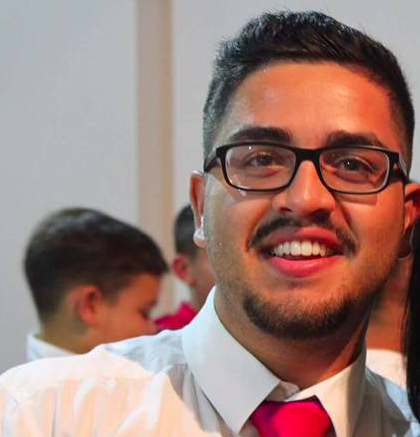
\includegraphics[width=20mm, height=20mm]{img/miguel.png} & Miguel Pinto & 79060\\
      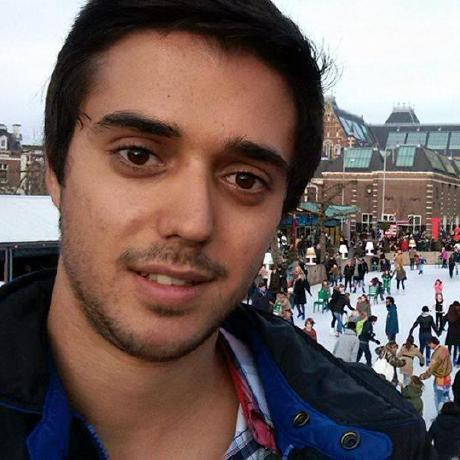
\includegraphics[width=20mm, height=20mm]{img/bernardo.jpeg} & Bernardo Casaleiro & 87827\\
      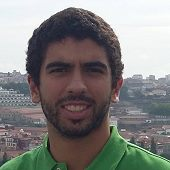
\includegraphics[width=20mm, height=20mm]{img/joao.jpeg} & João Godinho & 87830\\
    \end{tabular}
    \vfill

    {\large \today\par}
  \end{center}
\end{titlepage}

\section{Problem}
First response emergency systems are a limited resource. Their usage makes a difference in life-or-death situations!
Requesting an ambulance is a serious matter.
It should be simple, secure, fast and first of all always available.
For that the Dispatch Center must be fault tolerant.

It should separate the real requests from the false ones and provide a response accordingly.
Improper usage must be detected to avoid misallocation of resources while real requests should
trigger an appropriate response.

\section{Requirements}

\subsection{Application Requirements}
\begin{enumerate}
  \item Send an emergency request.
  \item Inform the estimated time for the user's request to be answered.
  \item \st{Confirm or deny if there is an emergency nearby.}
\end{enumerate}

\subsection{Server Requirements}
\begin{enumerate}
  \item Receive a request
  \item Insert a request in a queue depending on the user rating.
  \item \st{Request confirmation from users nearby the emergency.}
  \item Log the requests.
  \item Send the expected response time.
  \item Send the confirmation that an ambulance is on route.
  \item Rate the user accordingly at the end of the request.
  \item Temporarily block a user for abusive usage.
\end{enumerate}

\subsection{Security Requirements}
\begin{enumerate}
  \item Non-repudiation.
  \item \st{Fault tolerance to DoS.}
  \item \st{Firewall, responsible for filtering the requests.}
  \item \underline{Filter, responsible for filtering the requests.}
  \item Auditing mechanisms.
  \item Secure channel between user and Dispatch Central.
\end{enumerate}

\section{Solution}



\section{Results / Implemented Solution}

\begin{figure}[ht]
    \centering
    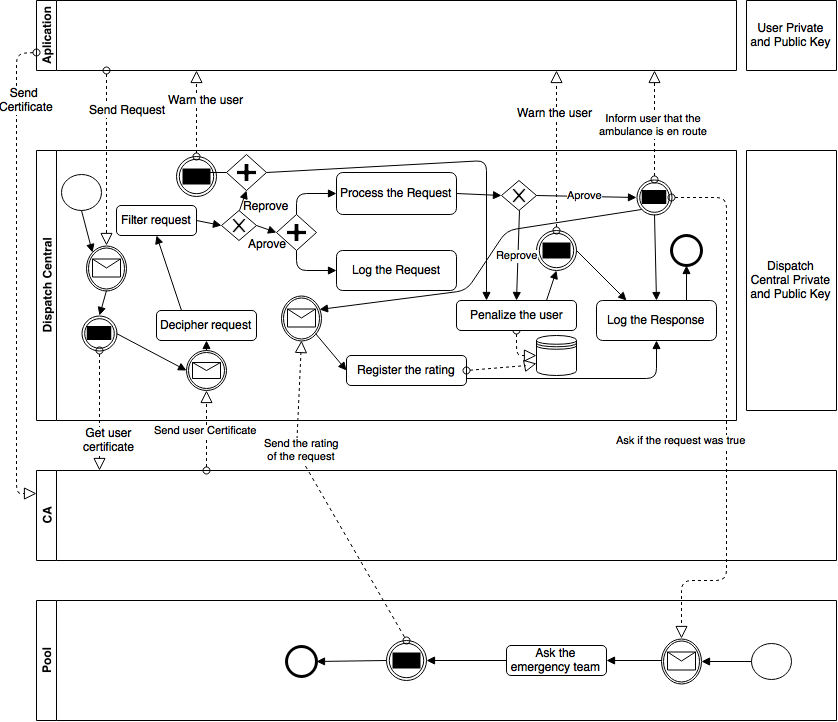
\includegraphics[scale=0.50]{img/advanced-solution.png}
\end{figure}

Our solution has two main components: the dispatch central and the user aplication.
In order to meet the security requirements we also implemented a certificate authority and a confirmation central.

The user aplication allow the user to send emergency requests. When starting the application it first sends
the user certificate to the certificate authority. Then the user is able to send requests to the dispatch central.

When receiving a request the dispatch central asks the CA for the user certificate in order to decipher the request and
passes it through a series of filters to exclude false ones. Only processing the accepted ones. The dispatch central then
notifies the user either that help is on the way or that the request sent was false and reminds the user of the consequences.
After an emergency team is dispatched the server asks the confirmation central if it was actually a real request.
If it wasn't the user is penalized.

All this comunications between the components are made using Java SSL Sockets in order to guarantee a secure channels and
always cyphered using the proper certificates provided by the certificate authority.

\section{Evaluation}
With our implementation we reached the majority of the security requirements proposed.

\section{Conclusion}

\section{References}

\subsection{Tool References}
\begin{description}
  \item [PostgreSQL] \href{https://www.postgresql.org}{Database to save the users.}
  \item [javax.net.ssl.SSLServerSocket] \href{https://docs.oracle.com/javase/7/docs/api/java/net/Socket.html}{Establish a secure connection.}
  \item [PostgreSQL JDBC] \href{https://jdbc.postgresql.org}{Driver to use PostgreSQL with Java.}
\end{description}

\end{document}
